\documentclass[11pt,a4paper]{article}
\usepackage{{../../paquete-formulas}}
\usepackage{{../../estilos-formulas}}

\newcommand{\materia}{Electrónica Industrial}

\begin{document}
	\pagestyle{pieyencabezado}
	\section*{Nomenclatura}
	
	\begin{tabular}{r l r l}
		$V_Z$ & jeje &&\\
	\end{tabular}
	\unidad{1}{Dispositivos de estado sólido}
	\begin{multicols}{2}
		\begin{cajita}
			hola jaja
		\end{cajita}
		
		
		\begin{cajita}
			chau jeje
		\end{cajita}
	\end{multicols}

	\begin{cajita}
		buen día
	\end{cajita}

	\unidad{2}{Transistores}
	
	\begin{multicols}{2}
		
		\begin{cajita}
			\subtitulo{Transistor bipolar BJT}
			\subsubtitulo{Tipo constructivo}
			\begin{tabular}{c c}
				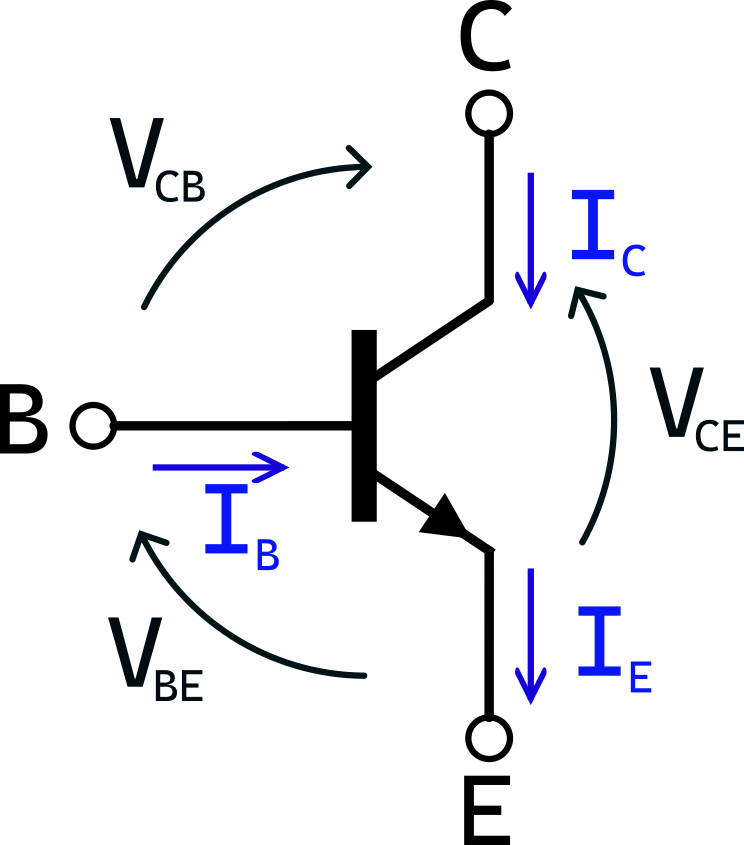
\includegraphics[width = .3\linewidth]{transistor-npn} & 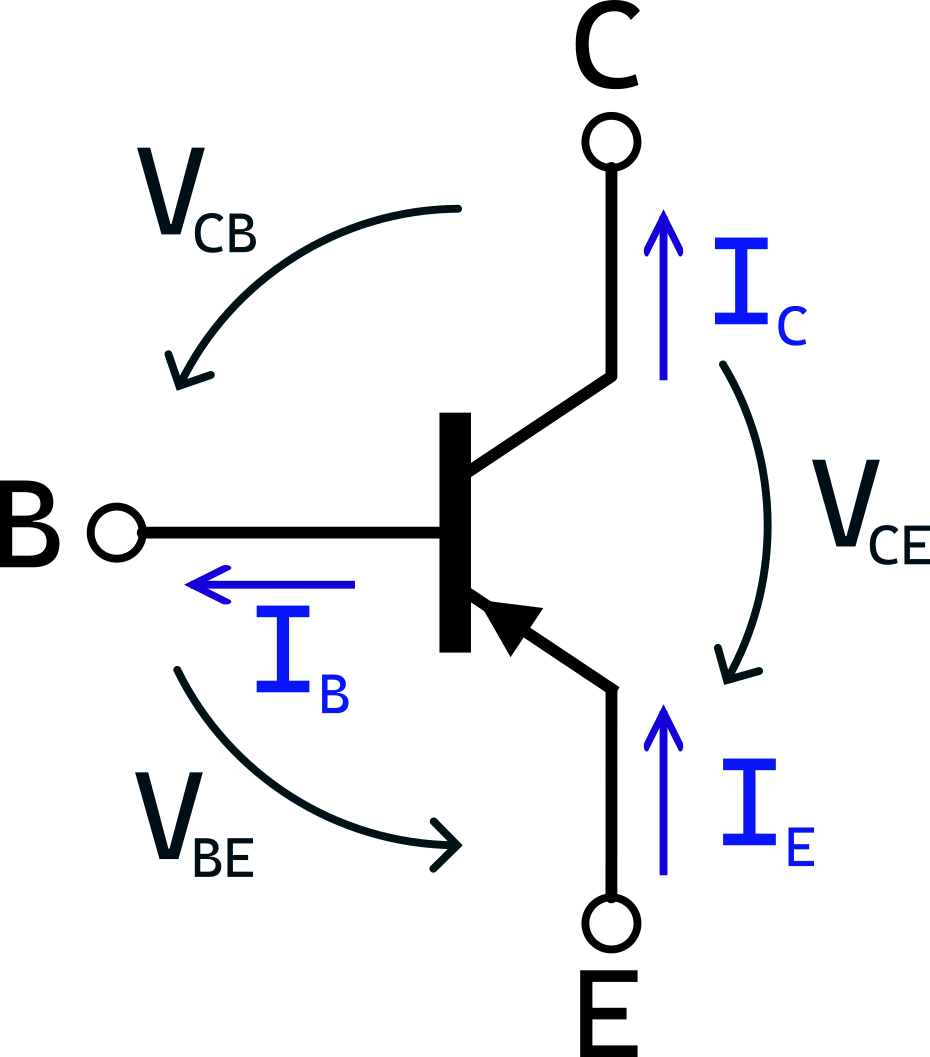
\includegraphics[width = .3\linewidth]{transistor-pnp} \\
				\textsc{npn} & \textsc{pnp} \\
				Sale corriente hacia E & Ingresa corriente a E
			\end{tabular}
			\subsubtitulo{Configuración}
			\begin{tabular}{c c c}
				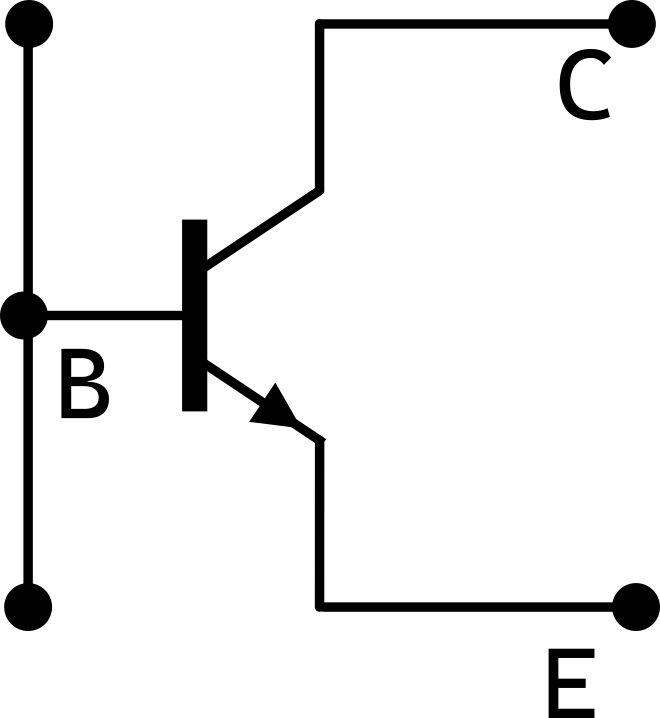
\includegraphics[width = .2\linewidth]{base-comun} & 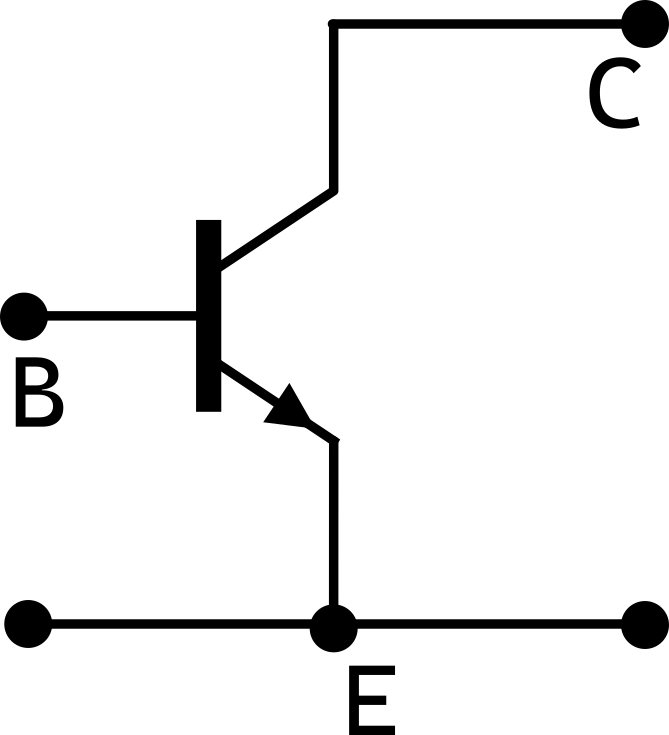
\includegraphics[width = .2\linewidth]{emisor-comun} & 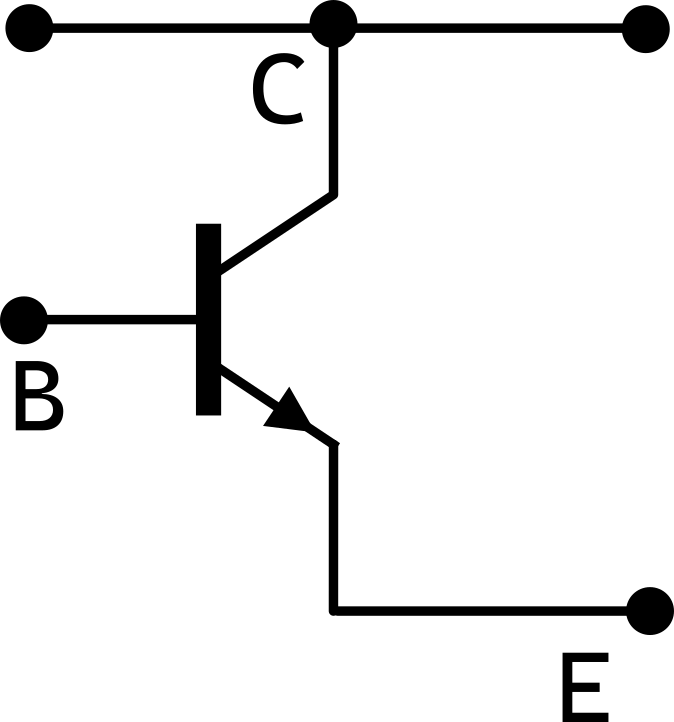
\includegraphics[width = .2\linewidth]{colector-comun} \\
				\textsl{Base común} & \textsl{Emisor común} & \textsl{Colector común}
			\end{tabular}
		\end{cajita}
	
	\columnbreak %Revisar después
	
		\begin{cajita}
			\subtitulo{Polarización del BJT}
			
			\subsubtitulo{Ecuaciones del dispositivo}\vspace{-.5cm}
					
			\begin{multicols}{2}
				\begin{tabular}{l}
					$I_C = \alpha I_E$ \quad;\quad
					$I_C = \beta I_B$ \\[.1cm]
					Si no se especifica: $\alpha = 1 $ \\[.1cm] 
					$V_{BB} = V_{R_B} + V_{BE}$ \\[.1cm] 
					$V_{CC} = V_{R_C} + V_{CE}$ \\[.1cm]
					$I_E = I_B + I_C$
				\end{tabular}
				\columnbreak
				
				img del esquema de un transistor con emisor común
			\end{multicols}	
			
			\subsubtitulo{Aplicación en conmutación}\vspace{-.3cm}
		
			Garantizar que: $\beta i_B = 5 i_C$\\
			\begin{tabular}{l l}
				\textbf{Corte} & \textbf{Saturación} \\[.1cm]
				$i_B = 0$ & $v_{CE} = 0.2 V$ \\[.1cm]
				$i_C = i_{fuga}$ & $i_C = \dfrac{V_{CC}}{R_C + R_E}$\\[.1cm]
				Interruptor abierto & $v_{CE} = V_{CC}$ \\[.1cm]
				Interruptor cerrado & \\
			\end{tabular}
	
			\subsubtitulo{Aplicación para amplificación}\vspace{-.8cm}
		
			\begin{flushleft}
				Condición para aplicar el método aproximado:
			\end{flushleft}
				$\beta R_E \geq 10 R_2$\\
		\end{cajita}

	\end{multicols}
\end{document}